\documentclass{article}

\usepackage[utf8]{inputenc}
\usepackage{graphicx}
\usepackage[german]{babel}
\usepackage{algpseudocode}
\usepackage{algorithm}
\usepackage{amsmath}
\usepackage{hyperref}

%\usepackage{algorithmic}
\usepackage{cite}

\setlength{\parindent}{0pt}

\title{Proteinsequenz-Vergleich mit KSEARCH und SANS}
\author{Meike Bruns, Florian Markowsky, Michael Spohn}

\begin{document}

\maketitle
\thispagestyle{empty}
\begin{abstract}
\end{abstract}
\newpage

\tableofcontents
\thispagestyle{empty}
\newpage

\section{Einleitung: Sequenzvergleiche}

Eine bei der Sequenzanalyse am häufigsten anfallenden Aufgaben ist der Vergleich
von Sequenzen. 
Sowohl bei DNA als auch bei Proteinsequenzen geben Sequenzvergleiche Aufschluss über die Ähnlichkeiten von Sequenzen, die dazu herangezogen werden, Verwandschaftsbeziehungen zwischen den einzelnen Sequenzen oder konservierte Regionen zu ermitteln. Bei unbekannten Proteinensequenzen lassen sich so beispielsweise Vorhersagen zur Funktion oder zur Struktur machen. Da exakte Sequenzvergleiche sehr zeitaufwendig sind, wurden verschiedene weniger exakte, dafür schnellere Algorithmen entwickelt.\\
Viele dieser Algorithmen basieren auf Sequenzalignments, wie der FASTA-Algorithmus \cite{FASTA} oder BLAST \cite{BLAST}, der sich als Standard für den Proteinvergleich etabliert hat.
Andere Algorithmen, wie z.B. USEARCH \cite{USEARCH} berechnen Ähnlichkeiten von Sequenzen dagegen unabhängig von Alignments anhand der Ähnlichkeiten von Feature-Vektoren. 
Feature-Vektoren einer Sequenz können z.B. die in ihr enthaltenen k-mere oder Substrings sein. 
Um die Ähnlichkeit zweier Sequenzen zu bestimmen, werden ihre Feature-Vektoren verglichen und daraus ein Ähnlichkeits-Score ermittelt.\\
Während alignmentbasierte Methoden für viele Zwecke eingesetzt werden können, sind Feature-Vektor basierte Scores hauptsächlich in Anwendungsbereichen wie der nearest-neighbor-Analyse vorteilhaft. 
Dadurch, dass sie ganz ohne Alignment auskommen, sind sie meist sehr schnell und lassen sich daher auch für große Datenmengen gut verwenden. 
Dass die berechneten Scores keine detaillierten Informationen darüber enthalten,
wo zwei Sequenzen gleich und wo verschieden sind, ist in nearest-neighbor-Analysen wie z.B. dem Clustering kein Nachteil. 
Hier ist vor allem von Interesse, dass hohe Scores ein verlässlicher Indikator für eine hohe Ähnlichkeit sind.\\
Im folgenden stellen wir unsere Implementierung zwei von J. Patrik Koskinen und Liisa Holm entwickelte Algorithmen - SANS (Suffix Array Neighborhood Search) und KSEARCH - vor, die Feature-Vektor basierte Scores für Protein-Sequenzpaare ermitteln. Koskinen und Holm erreichten mit SANS für Proteinsequenzen, deren Sequenzidentität zwischen 50 und 100\% lag, eine mit Blast vergleichbare Sensitivität. Dieses Ergebnis ist für die Vergleiche von Proteinsequenzen überraschend, denn wegen der hohen Mutationswahrscheinlichkeiten einzelner Aminosäuren werden in BLAST zur Bestimmung von Ähnlichkeiten zwischen Proteinen Substitutionsmatrizen verwendet, die die Mutationswahrscheinlichkeiten der Aminosäuren in die Ähnlichkeitsberechnung einbeziehen. 
Diese Anpassung ist bei den vorgestellten Algorithmen nicht möglich.
%TODO und für KSEARCH? für mich sieht es bei k= 5 und k=6 ähnlich aus... in FIG 5...


\section{Algorithmen \& Implementierung}

\subsection{KSEARCH}
\label{ksearch}

Der in \cite{Holm} vorgestellte KSEARCH-Algorithmus ermittelt Ähnlichkeitsscores für Proteinpaare anhand der k-mere, die in den Sequenzen beider Proteine vorkommen. Für jedes mögliche k-mer der Länge $k$ wird die Häufigkeit seines Auftretens im query-Protein mit der Häufigkeit seines Auftretens im database-Protein multipliziert. Die Summe dieser Produkte über alle k-mere ergibt den KSEARCH-Score:

\begin{equation}
KSEARCH(query,database) = \sum_{w \in \mathcal A^k} G_k(query)(w) \cdot G_k(database)(w)
\end{equation}  
\textit{mit $G_k(query)(w)$ = Häufigkeit des Vorkommens des k-mers $w$ im query-Protein}\\ \\

Koskinen und Holm benutzen zu Berechnung der KSEARCH - Scores Suffixarrays, und erreichen so eine theoretische Laufzeitkomplexität von $O(|q_1..q_n| \cdot |d_1..d_n|)$, also in der Gesamtlänge der query- und database-Proteine. Laut Koskinen und Holm liegt der Vorteil der Implementierung mit Suffixarrays darin, dass der Parameter für $k$ frei gewählt werden kann. \\
%TODO Wie berechnen Koskinen und Holm den KSERACH SCORE??"The KSEARCH algorithm checks all instances of k-mers in the database, and the number of these instances %grows proportionally to the size of the database" [Seite 440]. \\
Mit der q-gram-Distanz existiert bereits ein Modell, dass auf der Idee basiert,
Sequenzpaaren anhand vom gemeinsamen k-meren (bzw. q-Worteni) Änhnlichkeitsscores zuzuweisen. 
Im Gegensatz zum KSEARCH Score ergibt sich der Score bei der q-gram-Distanz aus der Summe der Differenzbeträge $|G_q(query)(w) - G_q(database)(w)|$ der Häufigkeiten der k-mere im query- und database-Protein. 
Bei der q-gram-Distanz konnte durch die Verwendung von q-Wort Profilen eine
Laufzeit von $O(|n|+|m|+\mathcal{A}^q)$ erreicht werden, wobei $|m|$ und $|n|$
die Längen der Proteine, $\mathcal{A}^q$ die Anzahl der möglichen q-Worte
darstellen \cite{GSA}. Es erschien uns daher sinnvoll, q-Wort-Profile auch für die Berechnung von KSEARCH-Scores zu nutzen.\\
Für das Erstellen eines k-mer- bzw. q-Wort-Profils wird jedes mögliche k-mer durch ein Integer codiert. Ein Array von der Größe $\mathcal{A}^k$ enthält an jeder Position $i$ die Anzahl des dazugehörigen k-mers mit dem Integercode $i$, und wird daher mit Null initialisiert. Durch eine geschickte Codierung können die Codes der einzelnen, in der Sequenz enthaltenen k-mere in konstanter Zeit ermittelt werden, so dass die Berechnung der k-mer-Profile in ${O(|q_1..q_n|)}$ erfolgt. Da der KSEARCH-Score zur Bewertung von Proteinsequenzpaaren genutzt werden soll, ergibt sich bei der Verwendung von Arrays zur Speicherung der k-mer Profile eine erforderliche Größe von $\mathcal{A}^k = 20^k$. Darüber hinaus sind die Proteinsequenzen relativ kurz, so dass die berechneten k-mer Profile nur spärlich besetzt sind. Daher nutzen wir Hashes, um die k-mer-Profile zu speichern. \\
Unsere Implementierung des KSEARCH-Algorithmus erhält die durch das genometool encseq encode konkatenierten und komprimierten query- und database-Proteinsequenzen als Eingabe. Mit dem genometools Modul GtKmercodeiterator werden zunächst die k-mere jedes query-Proteins extrahiert und mit der genometools Funktion GtHashmap in einem Hash gespeichert.
Dann wird für jedes database-Protein das k-mer-Profil als hash angelegt und der KSEARCH-Score mit allen query-Poteinen ermittelt und ausgegeben. Da das k-mer-Profil des database-Proteins nicht noch einmal gebraucht wird, braucht es nicht gespeichert zu werden. Das Berechnen des k-mer-Profils eines database-Proteins $d$ geschieht in $O(|d|)$, für alle database-Proteine also in $O(d_1..d_n)$. Dazu kommt die Berechnung der KSEARCH-Scores, die, da das k-mer Profil als Hash vorliegt, für ein einzelnes Proteinpaar linear in der Anzahl unterschiedlicher k-mere im database-Protein $O(kVariety(d))$ ist, für alle Proteinpaare also in $O(|D| \cdot |Q| \cdot kVariety(d))$ liegt. Insgesamt erhalten wir also eine Laufzeitkomplexität von $O(|q_1..q_n|+|d_1..d_n|+|D| \cdot |Q| \cdot kVariety(d))$.



%\begin{algorithm}
%  \caption{Pseudocode unserer KSearch-Implementierung}
%\begin{algorithmic}
%  \Function{KSEARCH}{query-proteins $Q$, database-proteins $D$}
%    \For{each query-protein $q$}  
%      \State calculate kmer-profile \Comment $O(|q|)$
%      \State store kmer-profile in hashtable
%    \EndFor \Comment $\mathbf{O(|q_1..q_n|)}$
%    \For{each database-protein $d$} 
%      \State calculate kmer-profile \Comment $O(|d|)$
%      \For{i in $Q$}
%        \State calculate $KSEARCH(d,q_{i})$ \Comment $O(kVariety(d))$   
%        \State output $KSEARCH(d,q)$
%      \EndFor \Comment $\mathbf{O(|Q| \cdot kVariety(d))}$
%    \EndFor   \Comment $\mathbf{O(|d_1..d_n|+|D| \cdot |Q| \cdot kVariety(d))}$  
%  \EndFunction \Comment overall time complexity: $\mathbf{O(|q_1..q_n|+|d_1..d_n|+|D| \cdot |Q| \cdot kVariety(d))}$
%\end{algorithmic}
%%\end{algorithm}

\subsection{SANS}
\label{sans}

Der SANS-Algorithmus bewertet Proteinpaare, deren Suffixe längste gemeinsame
Präfixe haben, mit einem positiven Score. Suffixarrays haben die Eigenschaft,
dass Suffixe, die im Suffixarray nebeneinanderliegen, typischerweise lange
gemeinsame Präfixe haben. Für die SANS-Scores wird diese Eigenschaft dahingehend
genutzt, dass Proteinpaare von query- und database-Proteinen, deren Suffixe im
Suffixarray nahe beieinander liegen, mit einem hohen Score bewertet werden.\\
Zur Berechnung der SANS-Scores werden zunächst alle query-Proteine $q_1..q_n$ konkateniert, ebenso alle database-Proteine $d_1..d_n$. 
Aus den konkatenierten Sequenzen werden die Suffixarrays \emph{Suffixarray$_Q$} und \emph{Suffixarray$_D$} erstellt. 
Nun wird für jeden Suffix \emph{suffix$_{qx}$} im \emph{Suffixarray$_Q$} die
Position $i$ im \emph{Suffixarray$_D$} ermittelt, an der der Suffix gemäß der lexikographischen Ordnung einzusortieren wäre. 
Ein Fenster der Größe $2h$ wird so über diese Position gelegt, dass es die $h$
Positionen vor und die $h$ Positionen nach dem hypothetisch einsortierten
\emph{suffix$_{qx}$} überdeckt. 
Anhand dieses Fensters werden die SANS-Scores aktualisiert: 
Jeder Suffix \emph{suffix$_{dy}$} eines Proteins $y$ im Fenster erhöht den SANS-Score-Zähler der dazugezugehörigen Proteinkombination $(query_x,database_y)$ um eins. \\
Wenn für alle Suffixe aus \emph{Suffixarray$_Q$} die Scores aktualisiert wurden, kann der SANS-Score ausgegeben werden.

Formal berechnet sich der \emph{SANS(query,database)} also folgendermaßen:\\

\begin{equation}
SANS(query,database) = \sum_{s \in suffixe_q} \sum_{j=-w}^{+w} id(database,Suffixarray_D[position_i(s)  +j].protein) 
\end{equation}

Mit der Identitätsfunktion

\begin{equation}
id(a,b)=\begin{cases}
  1,  & if~a=b\\
  0,  & if~a\ne b\\
\end{cases}
\end{equation}

Koskinen und Holm setzen die Fenstergröße h standardmäßig auf die Größe der als
Ausgabe gewünschten Anzahl von Proteinpaaren pro query Protein. 
Das Ziel dabei ist es, jedem der ausgegebenen h Proteine, die Möglichkeit zu
geben, im Fenster aufzutauchen, selbst wenn die Suffixe \emph{suffix$_{d}$}
aller h Proteine beispielsweise vor der Position $i$ des Suffixes
\emph{suffix$_{qx}$} auftauchen. 
Da wir mehrere Ausgabevarianten implementieren, haben wir uns dagegen entschieden, den Standardwert für h an die Ausgabe zu koppeln.\\
Zum Erstellen der Suffixarrays aus den query- und database-Proteinen nutzen wir
den in den genometools enthaltenen Suffixerator, dessen Laufzeitkomplexität
linear in der Länge der konkatenierten Proteinsequenzen $O(|d_1..d_n|+|q_1..q_n|)$ ist.
Die Suffixarrays stellen die Eingabe für unseren SANS-Algorithmus dar.
%TODO ECHT?? -> Laufzeit. 
Da die endgültigen Scores erst feststehen, wenn alle Suffixe im
\emph{Suffixarray$_Q$}
verarbeitet wurden, muss zur Ermittelung der Scores eine Scorematrix der Größe
$|Q|\cdot|D|$ angelegt und mit Null initialisiert werden, wobei $|Q|$ die Anzahl
der query-, $|D|$ die Anzahl der database-Proteine beschreibt. Dies benötigt
$O(|Q|\cdot|D|)$ Zeit. Jetzt ermitteln wir die Positionen der Suffixe
i\emph{Suffix$_{qx}$} in \emph{Suffixarray$_D$}. Dazu laufen wir einmal durch
den gesamten \emph{Suffixarray$_Q$}. Da die Suffixe in den Suffixarrays
lexikographisch geordnet sind, brauchen wir nicht für jeden \emph{Suffix$_{qx}$}
durch den gesamten \emph{Suffixarray$_D$} zu laufen, sondern können mit der
Suche nach der Position von \emph{Suffix$_{qx}$} an der Position beginnen, an
der wir auch \emph{Suffix$_{qx-1}$} eingeordnet haben. Diese Position merken wir
uns in der Variablen \emph{position}. Damit laufen wir einmal durch den gesamten
\emph{Suffixarray$_Q$} sowie insgesamt genau einmal durch den gesamten
\emph{Suffixarray$_D$} und bleiben so in $O(|q_0..q_n| + |d_0..d_n|)$.
Zusätzlich müssen immer, wenn wir eine Position gefunden haben, die Scores $2
\cdot h$ Proteinpaaren in konstanter Zeit aktualisiert werden, so dass sich für
die Berechnung der Scores eine Laufzeit von ${O(|q_0..q_n|\cdot2h +
|d_0..d_n|)}$ ergibt. Zusammen erhalten wir also eine Laufzeitkomplexität von ${O(|q_0..q_n|\cdot2h + |d_0..d_n|+|Q|\cdot|D|)}$


%\begin{algorithm}
%  \caption{Pseudocode unserer SANS-Implementierung}
% \begin{algorithmic}
%   \Function{SANS}{$query proteins Q, database proteins D, windowsize h$}
%     \State calculate $suffixarray_Q$ for query proteins \Comment $O(|d_1..d_n|)$
%     \State calculate $suffixarray_D$ for database proteins \Comment $O(|q_1..q_n|)$
%     \State initialize score matrix \Comment $O(|Q|\cdot|D|)$
%     \State initialize $position = 0$
%     \For{each $suffix_{qx}$ from 0 - $suffixarray_Q$.length}
%       \State  $position$ = \Call {findPosition}{$suffix$, $suffixarray_D$, $position$} 
%       \State shift $2h$ window over $position$ 
%       \For{each $suffix_{dx}$ in window}
%         \State update SANS-scores for  $(q_x,d_x)$
%       \EndFor \Comment $\mathbf{O(2h)}$
%     \EndFor \Comment $\mathbf{O(|q_0..q_n|\cdot2h + |d_0..d_n|)}$
%    \EndFunction  \Comment{overall time complexity:$\mathbf{O(|q_0..q_n|\cdot2h + |d_0..d_n|+|Q|\cdot|D|)}$}   \\
%    
%    \Function{findPosition}{$suffix$, $suffixarray_D$, $position$}
%      \For{$i$ in $position$..$suffixarray_D$.length}
%        \If{$suffix$ fits in $suffixarrax_D[i]$}
%          \State return $i$ 
%        \EndIf
%      \EndFor 
%    \EndFunction
%  \end{algorithmic}
%\end{algorithm}

\subsection{Software Architektur}

\subsubsection{Genome Tools}

Die Genome Tools sind eine freie Sammlung von Tools, Klassen und Modulen zum
Analysieren von Genomen und zur Entwicklung weiterer Programme zur Genomanalyse \cite{gtools}. Wir implementierten die Algorithmen SANS und KSEARCH innerhalb der GenomeTools-Umgebung und nutzten dabei folgende der durch GenomeTools bereitgestellten Funktionalitäten:

\paragraph{GtToolbox}
Die GtToolbox ist eine Klasse, die die einzelne Tools enthält. Sie besitzt
Methoden zum parsen der übergebenen Parameter und zum Aufrufen des ausgewählten
Tools. Wir implementierten unsere Algorithmen SANS und KSEARCH als Tools
innerhalb der GtToolbox gt\_seqscore. 

\paragraph{GtEncseq}
GtEncseq encode ist ein Tool, um aus ein oder mehreren Sequenzdateien ein
GtEncseq-Objekt zu erzeugen. Ein Objekt der Klasse GtEncseq besteht aus den
konkatenierten und durch bit-Kompression codierten Sequenzen der Eingabedateien.
Je nachdem, welche Funktionalitäten für ein GtEncseq-Objekt gewünscht werden, werden pro Objekt bis zu vier Dateien angelegt. Mit den verschiedenen Funktionen der GtEncseq-Klasse lassen sich unterschiedliche Eigenschaften der codierten Sequenzen abfragen. Wir verwenden GtEncseq-Objekte als Eingabe für den KSEARCH-Algorithmus.

\paragraph{GtKmercodeiterator}
Der GtKmercodeiterator ist eine Klasse, deren Instanzen unter anderem ein GtEncseq-Objekt, eine Startposition und eine Länge für k erhalten. Mit den Klassenfunktionen gt\_kmercodeiterator\_encseq\_next() wird das jeweils nächste k-mer der GtEncseq als GtKmercode zurückgegeben. Wir benutzen diese Funktionalität, um die k-mer-Hashes für den KSEARCH-Algorithmus zu erstellen.

\paragraph{GtRankedList und GtRankedListIter}
Die Instanzen der GtRankedList-Klasse sind dynamische Listen fester Größe. In ihnen wird gewährleistet, dass die gespeicherten Objekte in der Liste jeweils die mit dem höchsten Rang sind. Die Größe der Liste sowie die Vergleichsfunktion zur Ermittlung des Ranges sind Klassenvariablen der GtRankedList, zur Eingabe von Objekten in die GtRankedList gibt es eine Klassenfunktion. Um alle in einerGtRankedList gespeicherten Objekte auszugeben, wird die GtRankedList an ein Objekt der Klasse GtRankedListIter übergeben.

\paragraph{GtHashmap}
Die Objekte der GtHashmap-Klasse sind Hashtables. Wir benutzen sie, um die k-mer
Profile der Proteinsequenzen zu speichern. Dabei stellt das jeweilige k-mer den
Schlüssel und die Anzahl des Auftretens des k-mers den zugeordneten Wert dar. Es
werden also nur Informationen über tatsächlich in der Sequenz vorkommende k-mere
gespeichert.

\paragraph{GtSuffixerator}
Der GtSuffixerator ist ein Tool, das aus einer Sequenzdatei oder einem GtEncseq-Objekt einen Suffixarray erstellt. Standardmäßig werden für einen Suffixarray fünf Dateien erstellt, zusätzlich können Dateien für die Burrow-Wheeler-Transformation oder den LCP-Table angelegt werden. Wir verwenden den GtSuffixerator, um aus den query- und database-Dateien Suffixarrays als Eingabe für den SANS-Algorithmus zu erstellen.

\subsubsection{Struktur}

Da wir zwei verschiedene Algorithmen implementieren, ist eine logische Trennung wichtig. Da beide jedoch eine ähnliche Funktionalität erfüllen und
zumindest teilweise gleiche Strukturen beinhalten, würde eine komplette Trennung auf Code-Redundanzen hinauslaufen. Um dieses Dilemma zu lösen, haben wir
die \emph{Seqscore} Toolbox geschaffen, die die beiden Tools \emph{KSEARCH} und \emph{SANS} enthält. Diese greifen auf die selbe Codebasis zu, 
\emph{bla\_seqscore.c}. Dabei ruft jedes Tool abhängig von den ihm übergebenen Ausgabeparametern einen Konstruktor in \emph{bla\_seqscore.c} auf. Es gibt also
sechs Konstruktoren, eine je Algorithmus und je gewählter Ausgabe. Siehe dazu Abbildung \ref{seqsc}. Auf diese Weise ist sichergestellt, das die 
Ergebnisstrukturen betreffender Code von beiden Algorithmen genutzt werden kann.

\begin{center}
  \begin{figure}
    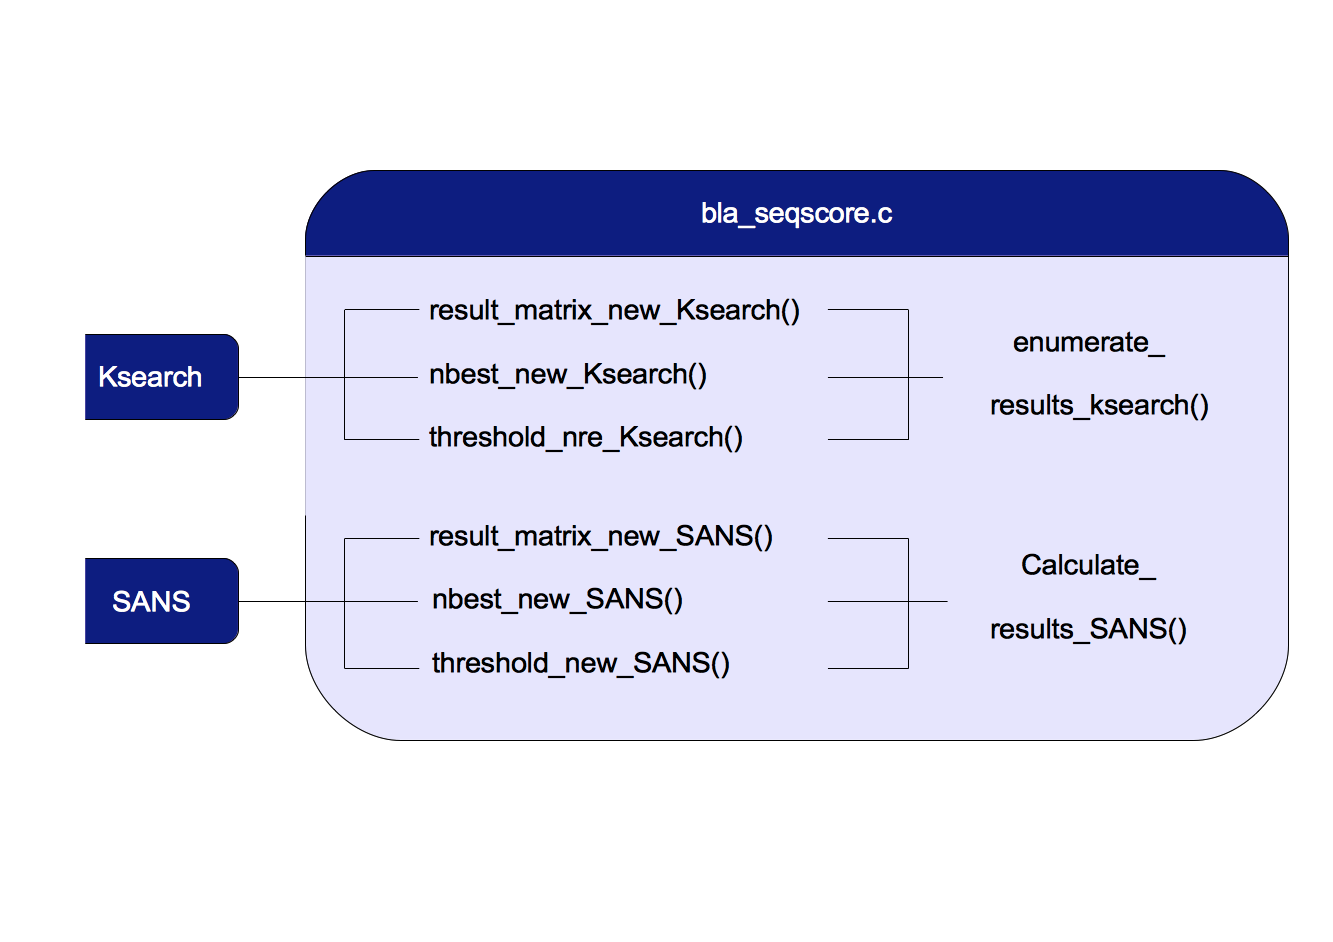
\includegraphics[width = \linewidth]{img/dia2}
    \caption{Struktur der \emph{bla\_seqscore.c}. Pro von Außen aufrufendem Tool sind drei Konstruktoren vorhanden, die jedoch jeweils wieder die
    selbe Berechnungsfunktion ausführen.}
    \label{seqsc}
  \end{figure}
\end{center}

\begin{center}
  \begin{figure}
    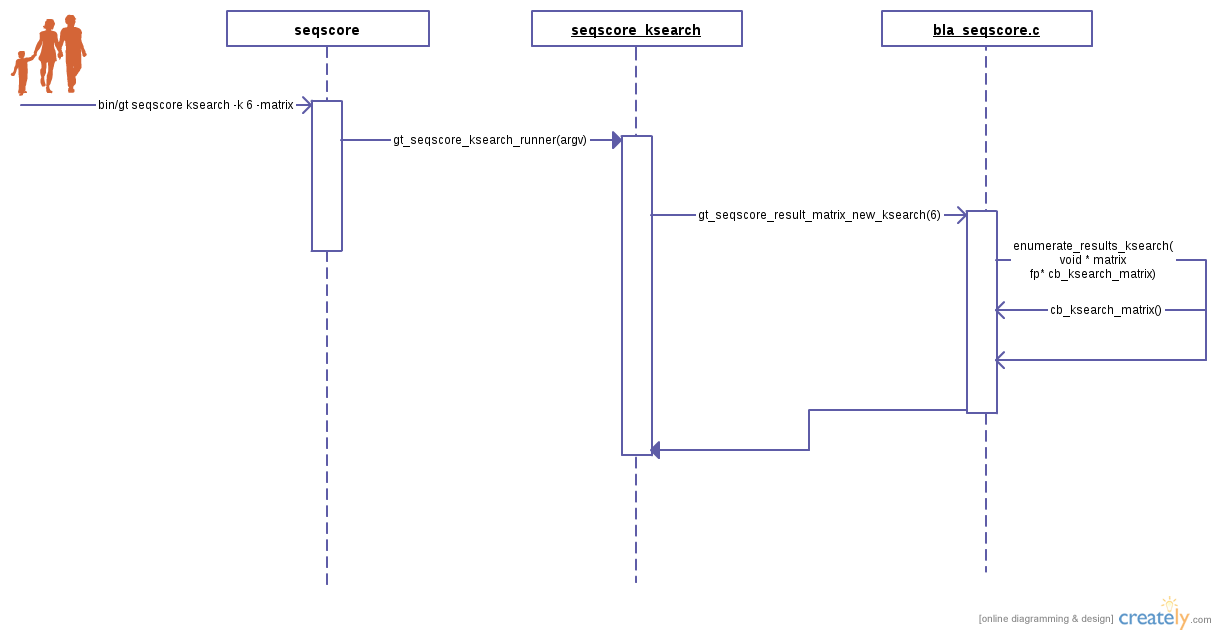
\includegraphics[width = \linewidth]{img/seqscore_seqence_fam.png}
    \caption{Sequenzdiagram der Abfolge der Funktionsaufrufe bei Aufruf von Ksearch mit -matrix Option. Die Aufrufe für die -nbest Option sind analog..}
    \label{manbes}
  \end{figure}
\end{center}

\begin{center}
  \begin{figure}
    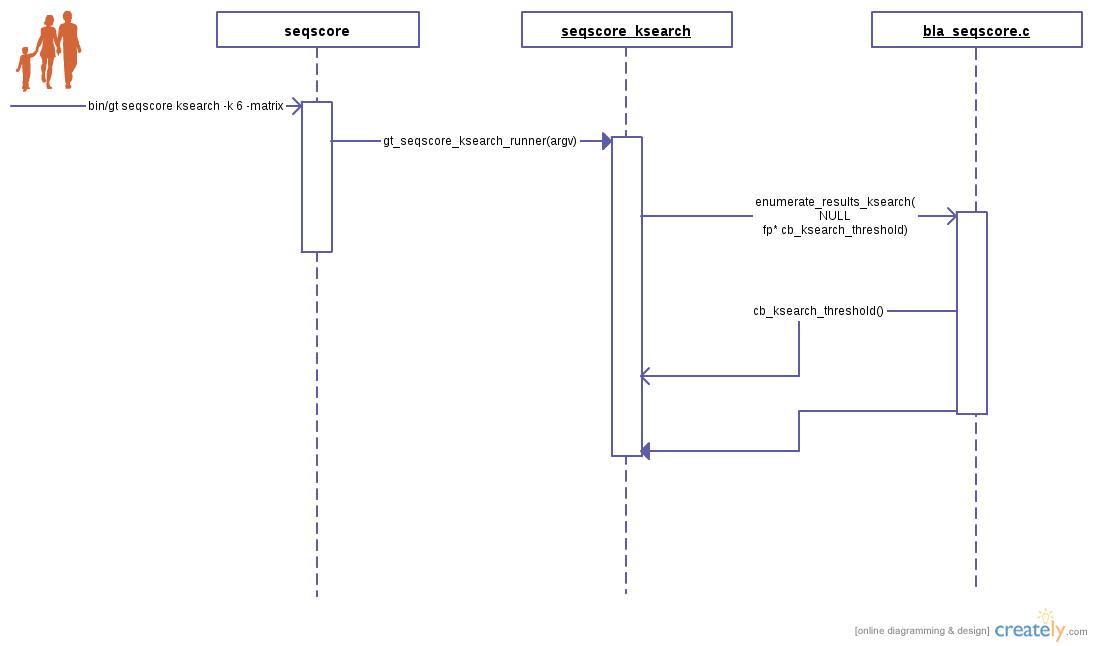
\includegraphics[width = \linewidth]{img/seqscore_sequence_fam_thresh.png}
    \caption{Sequenzdiagram der Abfolge der Funktionsaufrufe bei Aufruf von Ksearch mit -threshold Option. Man beachte, dass beim Aufruf der Funktion
      enumerate\_results\_ksearch() ein NULL-Pointer statt einer Ergebnisstruktur übergeben wird, da Scores, die über dem Grenzwert liegen, sofort ausgegeben
      werden, ohne in einer Datenstruktur gespeichert zu werden.}
    \label{thresh}
  \end{figure}
\end{center}

Pro Algorithmus wurde eine tatsächliche Berechnungsfunktion implementiert. Auf diese wird aus den drei Ergebnisstruktur abhängigen Konstruktoren des jeweiligen
Algorithmus zugegriffen. Wir gehen zunächst auf den \emph{SANS} Algorithmus ein.

Da durch die unter Abschnitt \ref{sans} vorgestellte Berechnungsvorschrift der
Score für ein Sequenzpaar erst bei der Terminierung des Algorithmus
fest steht, muss für jeden \emph{SANS} Lauf die gesamte Ergebnismatrix der Dimension $|Q|\cdot|D|$ mitgeführt werden. Die Konstruktoren 
\emph{result\_matrix\_new\_sans()}, \emph{nbest\_new\_sans()} und  \emph{threshold\_new\_sans()} definieren also jeweils die Ergebnismatrix und allokieren
den entsprechenden Speicher und rufen dann die \emph{calculate\_results\_sans()} Funktion auf, die die Matrix füllt. Anschließend werden die Daten 
wiederum konstruktorspezifisch aufbereitet. Der \emph{matrix}-Konstruktor wird also die gesamte Matrix, der \emph{nbest}-Konstruktor eine
Liste der $n$ besten Scores und der dazugehörigen Sequenzen und der \emph{treshold}-Konstruktor alle Sequenzpaare, deren Score über dem gegebenen
Schwellwert liegt, zurückgeben.

Wie in Abschnitt \ref{ksearch} ersichtlich, kann beim \emph{KSEARCH}-Algorithmus Speicherplatz gespart werden, da die Scores der Sequenzpaare
nacheinander ausgerechnet werden. Es muss also nur wenn der Benutzer die \emph{matrix}-Rückgabe gewünscht hat tatsächlich der Speicher für die
ganze Ergebnismatrix allokiert werden. Dies nutzen wir aus, indem die Konstruktoren \emph{result\_matrix\_new\_ksearch()}, \emph{nbest\_new\_ksearch()} 
und  \emph{threshold\_new\_ksearch()} eine ausgabespezifische Ergebnisstruktur erstellen und neben dieser Struktur auch eine Callback-Funktion an 
die \emph{enumerate\_results\_ksearch()} Funktion übergeben. Wie der Name der Funktion bereits anzeigt, berechnet die Funktion due \emph{KSEARCH}-Scores
sequenziell und ruft für jeden berechneten Score die übergebene Callback Funktion auf. Dieser wird auch die Ergebnisstruktur übergeben, so dass diese
der gewünschten Ausgabe entsprechend gefüllt werden kann. Abbildungen
\ref{manbes} und \ref{thresh} zeigen Sequenzdiagramme, die die
Reihenfolge und Struktur der Aufrufe und der entsprechenden Datanstrukturen am
Beispiel des \emph{nbest\_new\_ksearch} bzw. des \emph{thresh\_new\_ksearch} Konstruktors.

%\begin{center}
%  \begin{figure}
%    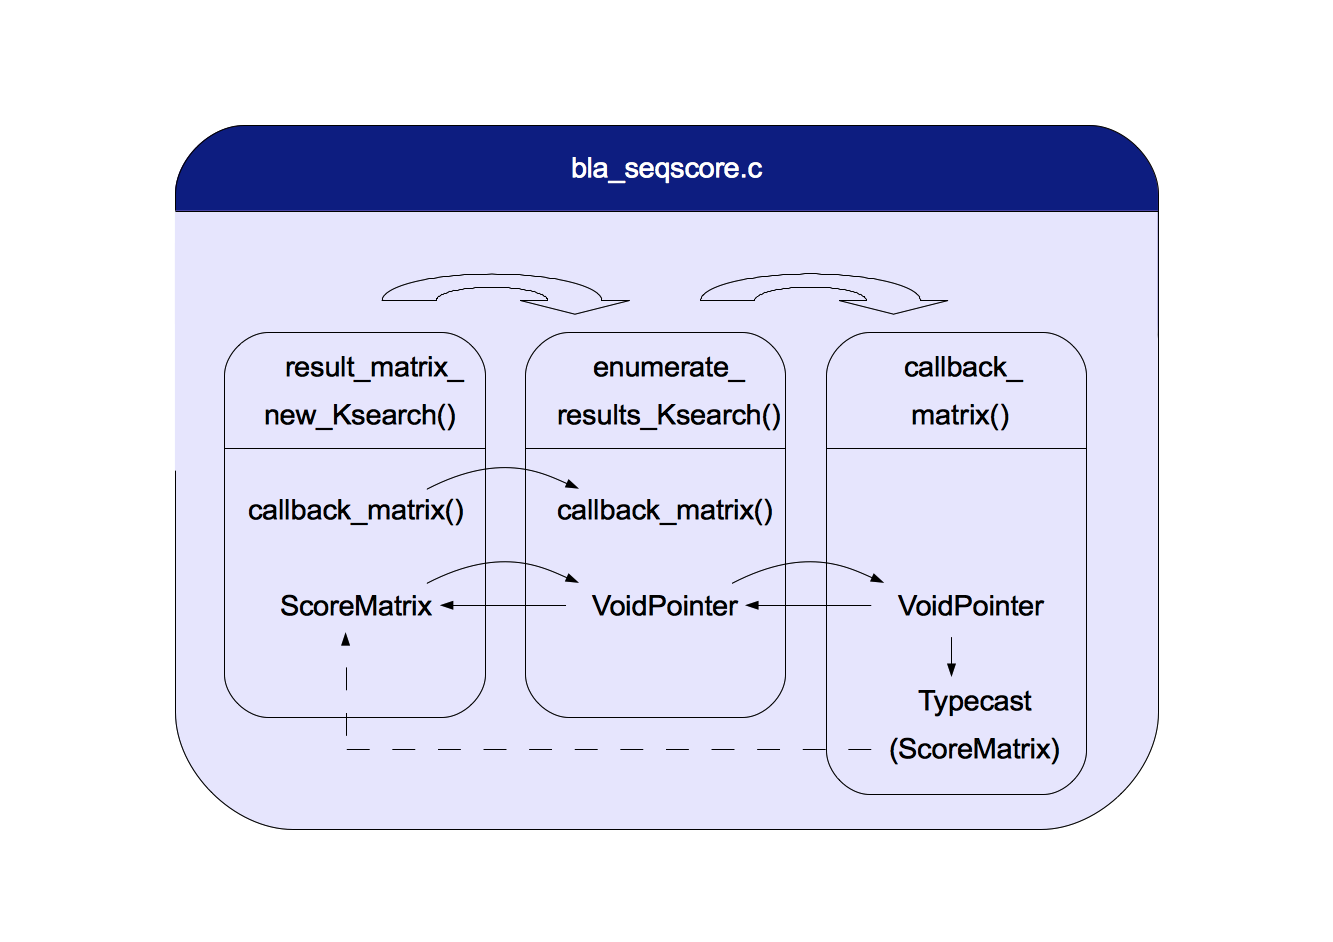
\includegraphics[width = \linewidth]{img/dia3}
%    \caption{Aufruf-Reiehenfolge bei Aufruf des \emph{result\_matrix\_new\_ksearch} Konstruktor. Der Konstruktor übergibt der Funktion zur Score-Berechnung
%      die Callback-Funktion \emph{callback\_matrix()} sowie die \emph{ScoreMatrix} als Ergebnisstruktur. Erst in der Callback-Funktion, die in der 
%      Berechnungsfunktion aufgerufen wird, wird die Ergebnisstruktur wieder zu einer Matrix gecastet und befüllt.}
%    \label{kscallback}
%  \end{figure}
%\end{center}

Für die \emph{matrix}-Option ist diese Rückgabestruktur ein einfaches zweidimensionales Array. Für die \emph{nbest} Option wurde eine in den genometools
bereits vorhandene Implementierung eines Red-Black-Trees als verkettete Liste genutzt. Diese kann schnell prüfen, ob ein neu generierter Score kleiner oder
größer als das bisher kleinste Element ist und entsprechend verfahren. Im Falle der \emph{threshold}-Option ist keine Ergebnisstruktur nötig,
da ein berechneter Score, der über dem gegebenen Schwellwert liegt, unmittelbar ausgegeben werden kann.

\section{Auswertung und Diskussion}

Um die erstellten Implementierungen von KSEARCH und SANS zu testen, wurden einerseits Laufzeitvergleiche mit den bereits existierenden Algorithmen aus \cite{Holm}, sowie Trefferquoten-Vergleiche mit bewährten Algorithmen wie SSEARCH und BLAST durchgeführt. Als Query-Datensatz dienten alle 1083 \textit{Rattus rattus}-Proteine aus der NCBI-Datenbank. Als Datenbank wurde die zur Uniprot gehörende Swissprot gewählt, welche ca. 500 000 Proteine enthält.

\subsection{Laufzeiten}

Die im Vergleich zu SSEARCH und BLAST sehr guten Laufzeiten des SANS-Algorithmus aus \cite{Holm}
konnten in unserer Implementierung nicht erreicht werden (Tab. \ref{runtimes}), sind jedoch für den praktischen Einsatz kurz genug.
Bei KSEARCH ist dies nicht der Fall. Ist die Laufzeit hier bei kleinen Test-Datensätzen noch vertretbar, steigt sie auf unserem realitätsnahen
Testdatensatz von 1083 Rattus-Proteinen mit der Swissprot Datenbank auf über 500 Minuten, was unsere KSEARCH Implementierung für den
praktischen Einsatz ungeeignet macht. Dabei wird der größte Teil der Zeit für Zugriffe auf den Hashtable aufgewendet (siehe Abschnitt \ref{ksearch}). Dies ist in sofern nicht
überraschend, dass wir uns aufgrund des massiven Speicherplatzbedarfs unserer ursprünglichen Implementierung für einen geringeren
Speicherplatzverbrauch entschieden, dafür jedoch bewusst Geschwindigkeitseinbußen in Kauf genommen haben.

Der implementierte SANS-Algorithmus benötigt lange für die Erstellung der Suffix-Arrays, zeigt jedoch bei zunehmender Fensterbreite \textit h 
eine weniger stark ansteigende Laufzeit als der Referenzalgorithmus. Mit Ausnahme des implementierten KSEARCH zeigen alle Algorithmen eine 
signifikante Verbesserung der Laufzeiten um teilweise mehr als 50 \%.
  \begin{table}[h]
    \caption{Laufzeitenvergleich; Holms entspricht den Algorithmen aus \cite{Holm}, MMF kennzeichnet die selbst implementierten Algorithmen; Berechnungen durchgeführt auf: Intel i5, 4*3.4GHz, 32gb RAM, XUbuntu}
    \begin{center}
    \begin{tabular}{lrrr}
    \hline
    Algorithmus & Indexing & Suche & Gesamt\\
    \hline
    BLAST & 0m12s & 27m23s & 27m35s\\
    SSEARCH & - & 60m0s & 60m0s\\
    KSEARCH Holms k6 & 1m29s & 0m14s & 1m43s\\
    KSEARCH MMF k6 & -  & 511m53s & 511m53s\\
    SANS Holms h16 & 1m29s &  0m15s & 1m44s\\
    SANS MMF  h16 & 14m19s & 0m36s & 14m55s\\
    SANS Holms h1000 & 1m29s & 7m7s & 8m36s\\
    SANS MMF  h1000 & 14m19s & 1m56s & 16m15s\\
    \hline
    \end{tabular}
    \label{runtimes}
    \end{center}
  \end{table}

\subsection{Scores}

Das wichtigste Kriterium bei der Beurteilung der Benutzbarkeit unserer Implementierungen ist die Qualität der Ergebnisse. Um hier Aussagen treffen
zu können, haben wir einerseits verglichen, wie viele der mit SSEARCH ermittelten Treffer auch mit den jeweiligen Algorithmen wiedergefunden werden konnten; 
andererseits wurde mittels AUC-Berechnungen die Effizienz der Algorithmen getestet.

\subsubsection{Vergleich mit SSEARCH}

%SANS
Um einen ersten Eindruck der Güte unseres SANS Algorithmen zu erhalten, verglichen wir zunächst die besten 1000 Scores unserer Implementierung
mit der aus \cite{Holm}. Dabei waren $919$ gleiche Sequenzpaare unter diesen am besten bewerteten $1000$. Es sind also $81$ sich unterscheidende
Sequenzpaare dabei. Generell konnten wir beobachten, das die gleichen Testsets nicht zu exakt gleichen Scores bei beiden Algorithmen führten. Die
Abweichungen, die wir hier feststellen konnten, waren jedoch im Vergleich zum Score gering.

Die Scores unterscheiden sich überhaupt, da einige Implementierungsdetails in \cite{Holm} nicht erschöpfend und nachvollziehbar beschrieben wurden,
und so an einigen Stellen eigene Entscheidungen getroffen werden mussten. Hier ist beispielsweise die Sortierung der Aminosäuren von Proteinsequenzen
zu nennen. Hier ist sowohl eine rein lexikographische als auch eine nach biologischen Kriterien vorgenommene Sortierung denkbar. Aus unterschiedlichen
Sortierungen resultiert dabei, dass Suffixe des querys an anderen stellen der Datenbank einsortiert werden. Somit ändern sich natürlich auch die 
entsprechenden Scores.

Weiterhin wurde, basierend auf \cite{Holm}, die Sensitivität beider Implementierungen verglichen. Dazu wurde zunächst SSEARCH auf den Rattus Query
Sequenzen mit der Swissprot Datenbank durchgeführt. Diese Referenzergebnisse wurden anschließend in den besten $1000$ Treffern der beiden SANS-Algorithmen
für jedes Query-Datenbank Paare gesucht. Wie in \cite{Holm} erfolgte eine Aufteilung in Identitätsklassen. Abbildung \ref{barplot} zeigt, dass beide
Implementierungen eine vergleichbare Sensitivität erreichen.

\begin{figure}
  \begin{center}
    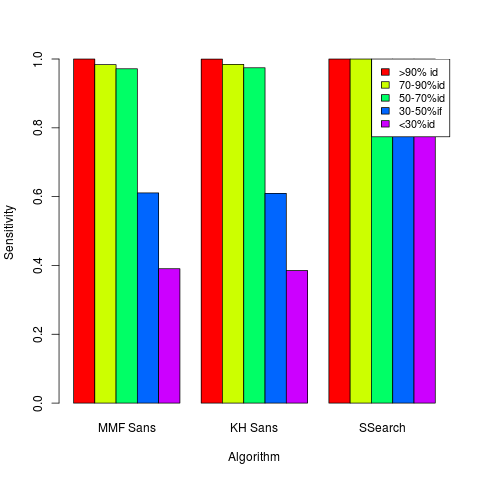
\includegraphics[width=0.6\textwidth]{img/barplot_beide.png}
    \caption{Sensitivität des selbst implementierten SANS-Algorithmus und dem aus \cite{Holm}. Als Referenz dienen SSearch-Alignments.
    Die Treffer sind nach Identität der Sequenzpaare eingeteilt.}
    \label{barplot}
  \end{center}
\end{figure}

\subsubsection{Area under the curve (AUC)}

Um die Effizienz eines Algorithmus zu ermitteln, wird ein precision-recall-Diagramm erstellt, und daraus die AUC berechnet. Die AUC ist die Fläche unter der Kurve, also das Integral. Das precision-recall-Diagramm erhält man, indem Präzision (precision) $p$ gegen Wiederfindungsrate (recall) $r$ geplottet wird. Um beide Werte zu erhalten, wird als erstes eine Liste \textit l mit einem Referenz-Algorithmus erstellt, und anschließend anhand dieser Liste \textit p und \textit r des zu testenden Algorithmus ermittelt.\\In Liste \textit l wurden alle BLAST-Treffer aus dem Query-Datensatz, welche einen e-Value niedriger als eins aufwiesen, eingetragen. Anschließend wurde mit jedem der ersten 50 Proteine des Query-Datensatzes einzeln eine Suche durchgeführt und die jeweils 50 besten Treffer \textit t ausgegeben. Für diese 50 Treffer wurden dann Präzision (precision) $p = \frac{t_0 ... t_i \in l}{t_0 ... t_i}$ und Wiederfindungsrate (recall) $r = \frac {t_0 ... t_i \in l}{t \in l}$ berechnet und ein precision-recall-Diagramm erstellt. Dabei gibt die Wiederfindungsrate \textit r an, wie viele der richtigen Treffer von \textit t zum Zeitpunkt \textit i bereits gefunden wurden. Die Präzision \textit p gibt die Anzahl der richtigen Treffer, im Verhältnis zu allen zum Zeitpunkt \textit i bereits betrachteten Treffern, an. Da \textit p und \textit r Werte zwischen 0 und 1 annehmen, hat die AUC im besten Fall den Wert 1. Im Allgemeinen nimmt mit zunehmender Wiederfindungsrate die Präzision ab, da bei einem kleinen AUC-Wert viele falsch Positiven Treffer auftreten, bis die maximale Anzahl aller richtig Treffer ermittelt ist. Je kleiner also der Wert für AUC, je ineffizienter ist der Algorithmus.\\Zu beachten ist, dass beim Plotten von \textit p gegen \textit r nur ein Punktdiagramm entsteht. Die darin enthaltenen Punkte können nicht interpoliert werden, wodurch die Kurve für die AUC nur näherungsweise bestimmt werden kann.\\Die Ergebnisse sind in Tab. 2 veranschaulicht.
  \begin{table}[h]
    \begin{center}
    \caption{Werte für die AUC; für die 50 ersten Proteine ; je höher der Wert, je effizienter arbeitet der     Algorithmus}
    \leftskip=-0.5cm
    \begin{tabular}{cccccccc}
      \hline
      \multicolumn{3}{c}{KSEARCH Holmes} & SANS Holmes &\multicolumn{3}{c}{KSEARCH MMF} & SANS MMF\\
      \cline{1-3}\cline{5-7}
      k = 5 & k = 6 & k = 7 & h = 50 & k = 5 & k = 6 & k = 7 & h = 50 \\
      \hline
      0,0000 & 0,0000 & 0,0000 & 0,0000 & 0,9663 & 0,9678 & 0,9677 & 0,9291 \\
      \hline
    \end{tabular}
    \end{center}
  \end{table}

\section{Anhang}

bla\_seqscore.h

\addcontentsline{toc}{section}{Literatur}
\bibliography{quellen}{}
\bibliographystyle{unsrt}

\end{document}
